
% plantilla obtenida de: https://www.overleaf.com/19886281jjqffwsxshmm#/73112823/

\documentclass[a4paper, 11pt]{article}
\usepackage{comment} % enables the use of multi-line comments (\ifx \fi) 
\usepackage{lipsum} %This package just generates Lorem Ipsum filler text. 
\usepackage{fullpage} % changes the margin

\usepackage[spanish]{babel}
\usepackage[utf8]{inputenc}
\decimalpoint
\usepackage{graphicx}

\usepackage{amsmath}
\usepackage{amsfonts}
% or
\usepackage{amssymb}
\usepackage{tikz}
\usepackage{array}
\newcolumntype{C}{>{$}l<{$}} % math-mode version of "l" column type
\newcommand{\imageins}[4]{\begin{figure}[!ht]		%Take the hardwork from using images. Let this command do the work for you. Insert images by just using this command \imageins{filename}{width as a ratio of total text width of the page}{caption name}{label name for referring in articles}		
    \centering
    \includegraphics[width=#2\textwidth]{#1}
    %\caption{#3}
    %\label{#4}
    \vspace{0.2em}
\end{figure}}

%%%%%%%%%%%%%%%%%%%%%%%%%%%%%%%%%%%%%%%%%%%%%%%%%%%%%%%%%%%%%%%%%%%%%%%%%%%%%%%%%%
\usepackage{listings}
\usepackage{color}
 
\definecolor{codegreen}{rgb}{0,0.6,0}
\definecolor{codegray}{rgb}{0.5,0.5,0.5}
\definecolor{codepurple}{rgb}{0.58,0,0.82}
\definecolor{backcolour}{rgb}{0.95,0.95,0.92}
 
\lstdefinestyle{mystyle}{
    backgroundcolor=\color{backcolour},   
    commentstyle=\color{codegreen},
    keywordstyle=\color{magenta},
    numberstyle=\tiny\color{codegray},
    stringstyle=\color{codepurple},
    basicstyle=\footnotesize,
    breakatwhitespace=false,         
    breaklines=true,                 
    captionpos=b,                    
    keepspaces=true,                 
    numbers=left,                    
    numbersep=5pt,                  
    showspaces=false,                
    showstringspaces=false,
    showtabs=false,                  
    tabsize=2
}
 
\lstset{style=mystyle}

%%%%%%%%%%%%%%%%%%%%%%%%%%%%%%%%%%%%%%%%%%%%%%%%%%%%%%%%%%%%%%%%%%%%%%%%%%%%%%%%%%

\begin{document}
%Header-Make sure you update this information!!!!
\noindent
\large\textbf{Práctica II} \hfill \textbf{Antonio Gámiz Delgado} \\
\normalsize Probabilidad \hfill 19 /11/2018
%\normalsize ECE 100-003 \hfill Teammates: Student1, Student2 \\
%Prof. Oruklu \hfill Lab Date: XX/XX/XX \\
%TA: Adam Sumner \hfill Due Date: XX/XX/XX

\section*{Ejercicio 2}
Sea $(X,Y)$ un vector aleatorio continuo con la función de densidad conjunta que se muestra a continuación:
\[
f(x,y)=\frac{4}{9}, \quad -2<x<-\frac{1}{2}, \quad x+2<y<1-x
\]
Obtener la función de densidad de $y$ condicionada a un valor $x_0$, así como la función de densidad de $x$ condicionada a un valor $y_0$. A través de esas funciones de densidad condicionadas, calcular $P(Y>1.07|X=-1.69)$ y $P(X<-1.69|Y=1.07)$. \\[0.1cm]

\begin{figure}[h]
\center
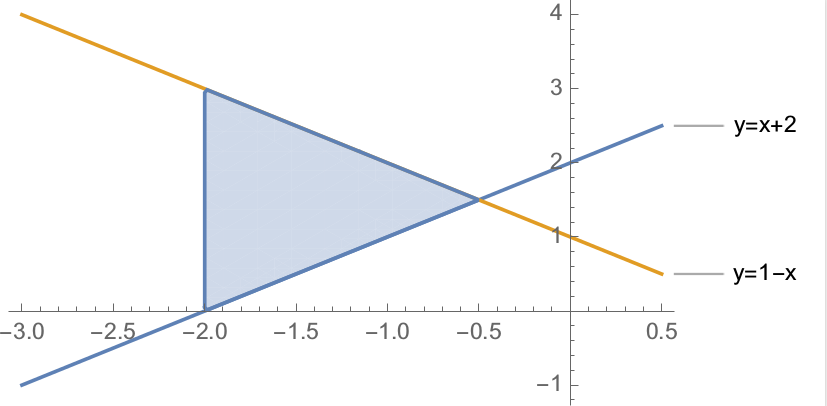
\includegraphics[scale=0.5]{area.png}
\caption{Área en la que vamos a trabajar.}
\end{figure}

Usando las restricciones $x+2<y<1-x$ y $-2<x<-0.5$ sabemos que $0<y<3$.

Calculamos ahora las funciones marginales asociadas a $x$ e $y$.
\[
f_1(x)=\int_{-\infty}^{+\infty}f(x,y)dy=\frac{4}{9}\int_{x+2}^{1-x}dy=\frac{4}{9}\left(1-x-x-2\right)=\frac{4}{9}\left(-2x-1\right), \quad -2<x<-\frac{1}{2}
\]

En el caso en el que $\frac{3}{2} < y < 3$ también tenemos que añadir el área que queda bajo $y=\frac{3}{2}$, que es la mitad del área del triángulo: $\frac{3*\frac{3}{2}}{2}=\frac{9}{4}$. Por lo que tenemos que sumar $\frac{9}{8}$.

\[
f_2(y)=\int_{-\infty}^{+\infty}f(x,y)dx=\left \{ \begin{array}{ll}
\displaystyle\frac{4}{9}\int_{-2}^{y-2}dx=\frac{4}{9}y & 0<y\leq\frac{3}{2}\\
\displaystyle\frac{4}{9}\left(\int_{\frac{3}{2}}^{y-1}dx+\frac{9}{8}\right)=\frac{4}{9}\left(y-\frac{5}{2}+\frac{9}{8}\right)=\frac{4}{9}\left(y-\frac{11}{8}\right)& \frac{3}{2} < y < 3

\end{array}\right.
\]

Ahora ya podemos calcular las funciones de densidad condicionadas:

\[
f(Y|X=x_0)=\displaystyle\frac{f(x_0,y)}{f_1(x_0)}=\frac{\frac{4}{9}}{\frac{4}{9}(-2x_0-1)}=-\frac{1}{2x_0+1}, \quad -2<x_0<-\frac{1}{2} \enskip x_0+2 < y < 1-x_0
\]

\[
f(X|Y=y_0)=\displaystyle\frac{f(x,y_0)}{f_2(y_0)} =\left \{ \begin{array}{ll}
\displaystyle\frac{1}{y_0} & 0 < y_0 \leq \frac{3}{2} \enskip -2 < x < -\frac{1}{2}\\
\displaystyle\frac{1}{y_0-\frac{11}{8}} & \frac{3}{2} < y_0 < 3 \enskip -2 < x < -\frac{1}{2}
\end{array}\right.
\]

Calculamos ahora la función de distribución condicionada:

\[
F\left(y_0|X=x_0\right)=\displaystyle\int_{x_0+2}^{y_0}-\displaystyle\frac{1}{2x_0+1}dy=\frac{x_0+2-y_0}{2x+1}, \quad -2<x_0<-\frac{1}{2}, \enskip x_0+2<y_0<1-x_0
\]
\[
F(x_0|Y=y_0) =\left \{ \begin{array}{ll}
\displaystyle\int_{-2}^{x_0}\frac{1}{y_0}dy=\frac{x_0+2}{y_0}, & -2 < x_0 < -\frac{1}{2} \enskip 0 < y \leq \frac{3}{2}\\
\displaystyle\int_{-2}^{x_0}\frac{1}{y_0-\frac{11}{8}}dy=\frac{x_0+2}{y_0-\frac{11}{8}}, & -2 < x_0 < -\frac{1}{2} \enskip \frac{3}{2} < y < 3
\end{array}\right.
\]
Ahora podemos calcular:
\[
P(Y>1.07|X=-1.69)=1-P(Y\leq 1.07|X=-1.69)=\frac{-1.69+2-1.07}{2(-1.07)+1}=\frac{2}{3}.
\]
\[
P(X<-1.69|Y=1.07)=F(-1.69|Y=1.07)=\frac{-1.69+2}{1.07}=\frac{31}{107}.
\]

\end{document}